
%packages
\usepackage{natbib}
\usepackage{amsmath}
\usepackage{amsthm}
\usepackage{mathtools}
\usepackage{mdframed}
\usepackage{subfigure}
\usepackage{booktabs}
% \usepackage{hyperref}
\usepackage{subfigure}
\usepackage{siunitx} % Provides the \SI{}{} and \si{} command for typesetting SI units
\usepackage{graphicx} % Required for the inclusion of images
% \usepackage{natbib} % Required to change bibliography style to APA
\usepackage{datetime}
\usepackage{lscape}
\usepackage{algorithm}
\usepackage{algorithmic}
\usepackage{xspace}
\usepackage[english]{babel} % English language/hyphenation
\usepackage{proof}
\usepackage{booktabs} % Top and bottom rules for tables
\usepackage[colorlinks, allcolors = blue,]{hyperref}
\usepackage{accents}
\usepackage{amsfonts}
\usepackage{stmaryrd}
\usepackage{amsmath,amsthm,amssymb,latexsym} 
\usepackage{microtype}
\usepackage{graphicx}
\usepackage{subfigure}
\usepackage{booktabs} % for professional tables
\usepackage{hyperref}
\usepackage{icml2019}
\usepackage{lipsum}

\usepackage{authblk}


%new commands
\newcommand{\theHalgorithm}{\arabic{algorithm}}
\newtheorem{definition}{Definition}
\usepackage{cancel}
\usepackage[normalem]{ulem}
\newcommand{\dataobs}{\textbf{x}}
\newcommand{\adj}[2]{\textbf{adj}(#1,#2)}
\newcommand{\candidateset}{\mathcal{R}_{\textup{post}}}
\newcommand{\bprior}{\boldsymbol{\beta}_{\textup{prior}}}
\newcommand{\bysinfer}{\mathsf{Infer}}
\newcommand{\betad}{\mathsf{Beta}}
\newcommand{\betaf}{\textup{B}}
\newcommand{\mbetaf}{\boldsymbol{\textup{B}}}
\newcommand{\vtheta}{\boldsymbol{\theta}}
\newcommand{\valpha}{\boldsymbol{\alpha}}
\newcommand{\vbeta}{\boldsymbol{\beta}}
\newcommand{\lapmech}{\mathsf{LSDim}}
\newcommand{\ilapmech}{\mathsf{LSHist}}
\newcommand{\binomial}[2]{\mathsf{Bin}(#1, #2)}
\newcommand{\multinomial}[2]{\mathsf{Mult}(#1, #2)}
\newcommand{\expmech}{\mathsf{EHD}}
\newcommand{\hexpmech}{\mathsf{EHDS}}
\newcommand{\lexpmech}{\mathsf{EHDL}}
\newcommand{\hexpmechd}{\mathsf{expMech}^{D}_{\hellinger}}
\newcommand{\privinfer}{\mathsf{PrivInfer}}
\newcommand{\hlg}{\mathsf{H}}
\newcommand{\dirichlet}[1]{\mathsf{Dir}(#1)}
\newcommand{\alphas}{\boldsymbol{\alpha}}
\newcommand{\xis}{\boldsymbol{\xi}}
\newcommand{\iverson}[1]{[#1]}
\newcommand{\datauni}{\mathcal{X}}
\newcommand{\hellinger}{\mathcal{H}}
\newcommand{\ux}[1]{u(\textbf{x}, {#1})}
\newcommand{\uxadj}[1]{u(\textbf{x}', {#1})}
\newcommand{\cardinality}[2]{\mathcal{C}^{#1}_{#2}}
\newcommand{\range}{\mathcal{O}}
\newcommand{\nomalizer}[1]{\sum\limits_{r'\in \mathcal{R}_{\textup{post}}} \exp \big(\frac{-\epsilon\cdot \mathcal{H} (\mathsf{BI}(#1),r')}{4 \cdot S(#1)}\big)}

\newcommand{\unomalizer}[1]{\sum\limits_{r'\in \mathcal{R}_{\textup{post}}} \exp \big(\frac{-\epsilon\cdot u(#1, r')}{4 \cdot S(#1)}\big)}


\newcommand{\hexpmechPr}[2]{\underset{z \thicksim \hexpmech(#1)}{\Pr}\left[ #2 \right]}
\newcommand{\lapmechPr}[2]{\underset{z \thicksim \lapmech(#1)}{\Pr}\left[ #2 \right]}

\newcommand{\ilapmechPr}[2]{\underset{
{z \thicksim \ilapmech(#1)}
}{\Pr}\left[ #2 \right]}

\newtheorem{thm}{Theorem}[section]

\newtheorem{lem}{Lemma}[section]

\newtheorem{assert}{Assertion}[lem]
\newcommand{\lap}[2]{\mathsf{Lap}(#1, #2)}
\newcommand{\todo}[1]{{\footnotesize \color{red}\textbf{[[ #1 ]]}}}

\title{\textbf{Notes of DP - Bayesian Inference}\\}
% \author{Jiawen \textsc{Liu}}
\date{\vspace{-10ex}}

\begin{document}
\maketitle

\section{Bayesian Inference Based on Dirichlet-Bernoulli Distribution}
\label{sec_bayesInfer}
In the Bayesian inference, first there is a prior distribution $\pi(\xis)$ to present our belief about parameter $\xis$. Then, we get some observed data $x$ sizing $n$, and produce a posterior distribution $Pr(\xis | x)$. The Bayesian inference is based on the Bayes' rule to calculate the posterior distribution:
\begin{equation*}
Pr(\xis | x) = \frac{Pr(x | \xis) \pi(\xis)}{Pr(x)}
\end{equation*}
It is denoted as $\bysinfer(x,\pi(\xis))$ taking an observed data set $x \in \mathcal{X}^n$ and a prior distribution $\pi(\xis)$ as input, outputting a posterior distribution of the parameter $\alphas$. For conciseness, when prior is given, we use $\bysinfer(x)$. $n$ is the size of the observed data size.

In our inference algorithm, we take a Dirichlet distribution as prior belief for the parameters, $\dirichlet(\alphas)$, where $\pi(\xis) = \dirichlet(\xis | \alphas) = \frac{\prod_{i = 1}^{m}\xi_i^{\alpha_i}}{B(\alphas)}$, and the Bernoulli distribution as the statistic model for $Pr(x | \alphas)$. $m$ is the order of the Dirichlet distribution.

We give a inference process based on a concrete example, where we throw an irregular $m$ sides dice. We want to infer the probability of getting each side $\xis$. We get a observed data set $\{s_{k_1}, s_{k_2}, \cdots, s_{k_n}\}$ by throwing the dice $n$ times, where $k_i \in \{1,2,\cdots, m\}$ denotes the side we get when we throw the dice the $i^{th}$ time. The posterior distribution is still a Dirichlet distribution with parameters $(\alpha_1 + n_1, \alpha_2 + n_2, \cdots, \alpha_m + n_m)$, where $n_i$ is the appearance time of the side $i$ in total.

In the case that $m = 2$, it is reduced to a Beta distribution $\betad(\alpha, \beta)$. The $m$ side dice change into a irregular coin with side $1$ and side $2$. The posterior is computed as $(\alpha + n_1, \beta + n_0)$, where $n_1$ is the appearance time of side $1$ in the observed data set and $n_0$ is the appearance time of the other side.



\section{Algorithm Setting up}
\label{sec_setup}
For now, we already have a prior distribution $prior$, an observed data set $x$.

\subsection{Exponential Mechanism with Global Sensitivity}
\label{subsec_emgs}

% \subsubsection{Mechanism Set up}

In exponential mechanism, candidate set $R$ can be obtained by enumerating $y \in \mathcal{X}^n$, i.e.
\begin{equation*}
R = \{\bysinfer(y)\ |\ y \in \mathcal{X}^n\}.
\end{equation*}

Hellinger distance $\hlg$ is used here to score these candidates. The utility function:
\begin{equation}
\label{equ_utility}
u(x,r) = -\hlg(\bysinfer(x), r); r \in R.
\end{equation}

Exponential mechanism with global sensitivity selects and outputs a candidate $r \in R$ with probability proportional to $exp(\frac{\epsilon u(x,r)}{2 \Delta_{g}u})$:
\begin{equation*}
P[r] = \frac
{exp(\frac{\epsilon u(x,r)}{2 \Delta_{g}u})}
{\Sigma_{r' \in R}\ exp(\frac{\epsilon u(x,r')}{2 \Delta_{g}u})},
\end{equation*}
where global sensitivity is calculated by:
\begin{equation*}
\Delta_{g}u = 
\max_{\{|x',y'| \leq 1;x',y'\in \mathcal{X}^n\}}\max_{\{r\in R\}}
|\hlg(\bysinfer(x'), r) - \hlg(\bysinfer(y'), r)|
\end{equation*}

The basic exponential mechanism is $\epsilon -$differential privacy\cite{dwork2014algorithmic}.

% We use probability proportional to $exp(\frac{\epsilon u(x,r)}{\Delta_{g}u})$ rather than $exp(\frac{\epsilon u(x,r)}{2 \Delta_{g}u})$. Since $\hlg$ is monotonic, i.e. our utility function is monotonic. 

% \subsubsection{Security Analysis}
% It can be proved that exponential mechanism with global sensitivity is $\epsilon$-differentially private. We denote the $\bysinfer$ with privacy mechanism as $\privinfer$. For adjacent data set $||x,y||_1 = 1$:
% \begin{equation*}
% \begin{split}
% \frac{P[\privinfer(x,u,R) = r]}{P[\privinfer(y,u,R) = r]}
% & =\frac
% {\frac
% {exp(\frac{\epsilon u(x,r)}{2 \Delta_{g}u})}
% {\Sigma_{r' \in R}\ exp(\frac{\epsilon u(x,r')}{2 \Delta_{g}u})}}
% {\frac
% {exp(\frac{\epsilon u(y,r)}{2 \Delta_{g}u})}
% {\Sigma_{r' \in R}\ exp(\frac{\epsilon u(y,r')}{2 \Delta_{g}u})}} \\
% & = \left(\frac
% {exp(\frac{\epsilon u(x,r)}{2 \Delta_{g}u})}
% {exp(\frac{\epsilon u(y,r)}{2 \Delta_{g}u})}
% \right)
% \cdot
% \left(\frac
% {\sum\limits_{r' \in R}\ exp(\frac{\epsilon u(y,r')}{2 \Delta_{g}u})}
% {\sum\limits_{r' \in R}\ exp(\frac{\epsilon u(x,r')}{2 \Delta_{g}u})}
% \right)\\
% & = exp\left(\frac
% {\epsilon (u(x,r) - u(y,r))}
% {2 \Delta_{g}u}
% \right)
% \cdot
% \left(\frac
% {\sum\limits_{r' \in R}\ exp(\frac{\epsilon u(y,r')}{2 \Delta_{g}u})}
% {\sum\limits_{r' \in R}\ exp(\frac{\epsilon u(x,r')}{2 \Delta_{g}u})}
% \right)\\
% & \leq
% exp(\frac{\epsilon}{2}) \cdot exp(\frac{\epsilon}{2}) \cdot
% \left(\frac
% {\sum\limits_{r' \in R}\ exp(\frac{\epsilon u(x,r')}{2 \Delta_{g}u})}
% {\sum\limits_{r' \in R}\ exp(\frac{\epsilon u(x,r')}{2 \Delta_{g}u})}
% \right)\\
% & = exp(\epsilon).
% \end{split}
% \end{equation*}

% Then, $\frac{P[\privinfer(x,u,R) = r]}{P[\privinfer(y,u,R) = r]} \geq exp(-\epsilon)$ can be obtained by symmetry.


\subsection{Exponential Mechanism with Local Sensitivity}
\label{subsec_emls}
% \subsubsection{Mechanism Set up}
Exponential mechanism with local sensitivity share the same candidate set and utility function as it with global sensitivity. This outputs a candidate $r \in R$ with probability proportional to $exp(\frac{\epsilon u(x,r)}{2 \Delta_{l}u})$:
\begin{equation*}
P[r] = \frac
{exp(\frac{\epsilon u(x,r)}{2 \Delta_{l}u})}
{\Sigma_{r' \in R}\ exp(\frac{\epsilon u(x,r')}{2 \Delta_{l}u})},
\end{equation*}

where local sensitivity is calculated by:

\begin{equation*}
\Delta_{l}u(x) = 
\max_{\{|x,y'| \leq 1;y'\in \mathcal{X}^n\}}\max_{\{r\in R\}}.
\hlg(\bysinfer(x), r) - \hlg(\bysinfer(y'), r)|
\end{equation*}

The exponential mechanism with local sensitivity is non differential privacy\cite{dwork2014algorithmic}.


\subsection{Exponential Mechanism with Smooth Sensitivity}
\label{sec_smoo}

\subsubsection{Algorithm Setting up}
The candidate set and utility function are still the same as before, differ only in the sensitivity. It will output a candidate $r \in R$ with probability proportional to $\exp(\frac{\epsilon u(x,r)}{2 S(x)})$:

\begin{equation*}
P[r] = \frac
{exp(\frac{\epsilon u(x,r)}{2 S(x)})}
{\Sigma_{r' \in R}\ exp(\frac{\epsilon u(x,r')}{2 S(x)})},
\end{equation*}
where the sensitivity in mechanism is smooth sensitivity $S(x)$\cite{nissim2007smooth}, calculated by:
\begin{equation*}
S_{\beta}(x) = \max(\Delta_{l}u(x), \max_{y \neq x; y \in D^{n}}(\Delta_{l}u(y)\cdot e^{-\beta d(x,y)})),
\end{equation*}
where $\beta = \beta(\epsilon, \delta)$. In our private Bayesian inference mechanism, we set the $\beta$ as $\ln(1 - \frac{\epsilon}{2 \ln (\frac{\delta}{2 (n + 1)})})$. 

\subsubsection{Sliding Property of Exponential Mechanism}
\begin{lem}
for any exponential mechanism $\expomech$, $\lambda = f(\epsilon, \delta)$, $\epsilon$ and $|\delta| < 1$, the sliding property holds:

\begin{equation*}
\underset{z \thicksim \expomech}{Pr}[u(r,x) = \hat{s}]
\leq
e^{\frac{\epsilon}{2}} \underset{z \thicksim \expomech}{Pr}[u(r,x) = (\Delta + \hat{s})] + \frac{\delta}{2},
\end{equation*}

\end{lem}

\begin{proof}
We denote the normalizer of the probability mass in $\expomech$: $\sum_{r' \in \mathcal{R}}exp(\frac{\epsilon u(r',x)}{2 S(x)})$ as $NL_x$:
\begin{equation*}
\begin{split}
LHS 
  = \underset{z \thicksim \expomech}{Pr}[u(r,x) = \hat{s}]
& = \frac{exp(\frac{\epsilon \hat{s}}{2 S(x)})}{NL_x}\\
& = \frac{exp(\frac{\epsilon (\hat{s} + \Delta - \Delta)}{2 S(x)})}{NL_x}\\
& = \frac{exp(\frac{\epsilon (\hat{s} + \Delta)}{2 S(x)} + \frac{- \epsilon \Delta}{2 S(x)})}{NL_x}\\
& = \frac{exp(\frac{\epsilon (\hat{s} + \Delta)}{2 S(x)})}{NL_x} \cdot e^{\frac{- \epsilon \Delta}{2 S(x)})}.\\
\end{split}
\end{equation*}

By bounding the $\Delta \geq -S(x)$, we can get:

\begin{equation*}
\begin{split}
\frac{exp(\frac{\epsilon (\hat{s} + \Delta)}{2 S(x)})}{NL_x} \cdot e^{\frac{- \epsilon \Delta}{2 S(x)}}
& \leq \frac{exp(\frac{\epsilon (\hat{s} + \Delta)}{2 S(x)})}{NL_x} \cdot e^{\frac{\epsilon}{2}}\\
&  =  e^{\frac{\epsilon}{2}} \underset{z \thicksim \expomech}{Pr}[u(r,x) = (\Delta + \hat{s})] \leq RHS\\
\end{split}
\end{equation*}

\end{proof}

\subsubsection{Dilation Property of Exponential Mechanism}
\begin{lem}
for any exponential mechanism $\expomech$, $\lambda < |\beta|$, $\epsilon$, $|\delta| < 1$ and $\beta \leq \ln(1 - \frac{\epsilon}{2 \ln (\frac{\delta}{2 (n + 1)})})$, the dilation property holds:

\begin{equation*}
\underset{r \thicksim \expomech}{Pr}[u(r) = z]
\leq
e^{\frac{\epsilon}{2}} \underset{r \thicksim \expomech}{Pr}[u(r) = e^{\lambda} z] + \frac{\delta}{2},
\end{equation*}
where the sensitivity in mechanism is still smooth sensitivity as above.
\end{lem}

\begin{proof}

The sensitivity is always greater than 0, and we are using $-\hlg(\bysinfer(x),r)$ for utility function, i.e., $u(r) \leq 0$, we need to consider two cases that $\lambda < 0$, and $\lambda > 0$:

We set the $h(z) = Pr[u(\expomech) = z] = \frac{exp(\frac{\epsilon z}{2 S(x)})}{NL_x}$.

We first consider $\lambda < 0$. In this case, $1 < e ^ {\lambda}$, so the ratio $\frac{h(z)}{h(e^{\lambda}z)} = \frac{exp(\frac{\epsilon z}{2 S(x)})}{exp(\frac{\epsilon (z \cdot e^{\lambda})}{2 S(x)})}$ is at most $\frac{\epsilon}{2}$.

Next, we proof the dilation property for $\lambda > 0$, The ratio of $\frac{h(z)}{h(e^{\lambda}z)}$ is $\exp(\frac{\epsilon}{2} \cdot \frac{u(\expomech) (1 - e^{\lambda})}{S(x)})$. Consider the event $G = \{ \expomech : u(\expomech) \leq \frac{S(x)}{(1 - e^{\lambda})}\}$. Under this event, the log-ratio above is at most $\frac{\epsilon}{2}$. The probability of $G$ under density $h(z)$ is $1 - \frac{\delta}{2}$. Thus, the probability of a given event $z$ is at most $Pr[z \cap G] + Pr[\overline{G}] \leq e^{\frac{\epsilon}{2}} Pr[e^{\lambda}z \cap G] + \frac{\delta}{2} \leq e^{\frac{\epsilon}{2}} Pr[e^{\lambda}z] + \frac{\delta}{2}$.\\


\textbf{Detail proof:}
\begin{itemize}

	\item $\lambda < 0$

		The left hand side will always be smaller than 0 and the right hand side greater than 0. This will always holds, i.e.
		\begin{equation*}
		\end{equation*}
	\item $\lambda > 0$


Because $\hat{s} = u(r)$ where $r \thicksim \expomech$, we can substitute $\hat{s}$ with $u(\expomech)$. Then, what we need to proof under the case $\lambda > 0$ is:
\begin{equation*}
u(\expomech) \leq \frac{S(x)}{(1 - e ^ {\lambda})}
\end{equation*}
By applying the accuracy property of exponential mechanism, we bound the probability that the equation holds with probability:
\begin{equation*}
\begin{split}
Pr[u(\expomech) \leq \frac{S(x)}{(1 - e ^ {\lambda})}] 
& \leq \frac{|\mathcal{R}|exp(\frac{\epsilon S(x)}{(1 - e ^ {\lambda})}/2 S(x))}{|\mathcal{R}_{OPT}| exp(\epsilon OPT_{u(x)}/2 S(x))}\\
\end{split}
\end{equation*}

In our Bayesian Inference mechanism, the size of the candidate set $\mathcal{R}$ is equal to the size of observed data set plus 1, i.e., $n + 1$, and $OPT_{u(x)} = 0$, then we have:
\begin{equation*}
\begin{split}
Pr[u(\expomech) \leq \frac{S(x)}{(1 - e ^ {\lambda})}] 
& = (n + 1)exp(\frac{\epsilon S(x)}{(1 - e ^ {\lambda})}/2 S(x))\\
& = (n + 1)exp(\frac{\epsilon}{2 (1 - e ^ {\lambda})})\\
\end{split}
\end{equation*}

When we set $\lambda \leq \ln(1 - \frac{\epsilon}{2 \ln (\frac{\delta}{2 (n + 1)})})$, it is easily to derive that $Pr[u(\expomech) \leq \frac{S(x)}{(1 - e ^ {\lambda})}] \leq \frac{\delta}{2}$.

\end{itemize}

\end{proof}

\section{Accuracy Analysis}
\subsection{Laplace Mechanism}

\subsection{Exponential Mechanism with Global Sensitivity}

\subsection{Exponential Mechanism with Local Sensitivity}

\subsection{Exponential Mechanism with Smooth Sensitivity}

\section{Experimental Evaluations}
\subsection{Computation Efficiency}
The formula for computing the local sensitivity is presented in Sec. \ref{subsec_emls}:$\max\limits_{\{|x,y'| \leq 1; y'\in \mathcal{X}^n\}}\max\limits_{\{r\in R\}} \{\hlg(\bysinfer(x), r) - \hlg(\bysinfer(y'), r)|\}$ can be reduced to $\max\limits_{\{|x,y'| \leq 1;y'\in \mathcal{X}^n\}}\hlg(\bysinfer(x), \bysinfer(y'))|$ by applying the distance triangle property. i.e., the maximum value over $\max\limits_{r \in R}$ always happen when $r = \bysinfer(x)$ itself, where $\Delta_{l}u(x) = \max\limits_{\{|x,y'| \leq 1;y'\in \mathcal{X}^n\}} \{\hlg(\bysinfer(x), \bysinfer(x)) - \hlg(\bysinfer(y'), \bysinfer(x))|\} = \max\limits_{\{|x,y'| \leq 1;y'\in \mathcal{X}^n\}} \{\hlg(\bysinfer(y'), \bysinfer(x))|\}$. We also have some experiments for validating our proposal as in Fig. \ref{fig_efficiency}, where we calculate the $\max\limits_{\{|x,y'| \leq 1;y'\in \mathcal{X}^n\}}$ value for every candidate $r \in R$. It is shown that maximum value taken when  $r = \bysinfer(x)$.

 \begin{figure}[h]
\centering
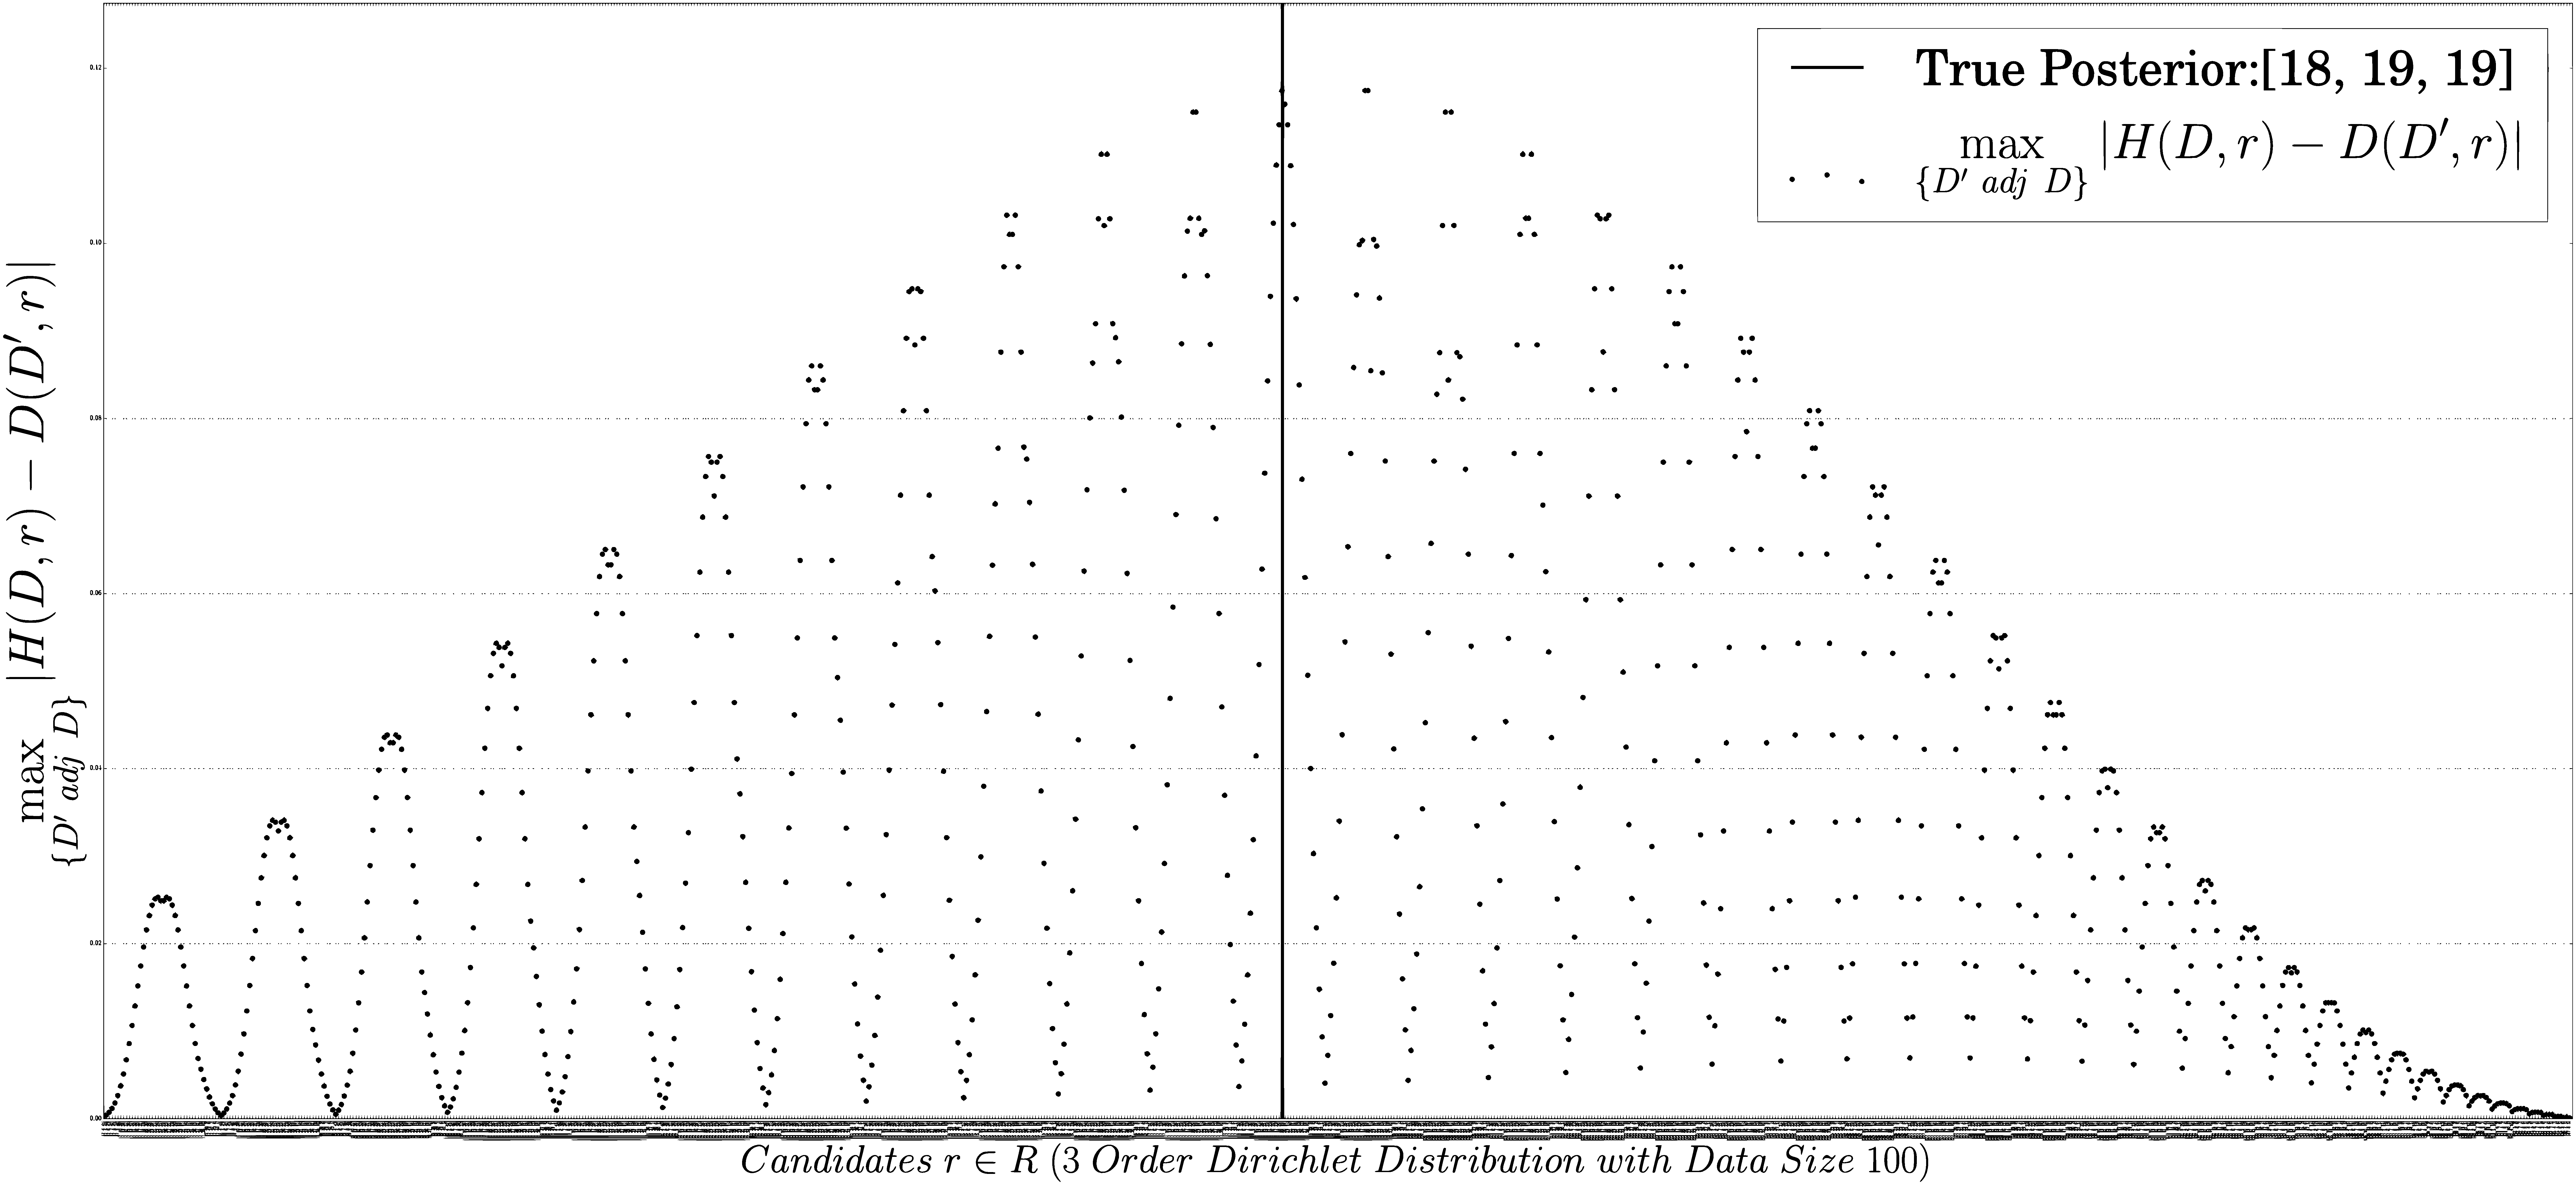
\includegraphics[width=1.0\textwidth]{efficiency}
\label{fig_efficiency}
\caption{Experimental Results for Finding the Local Sensitivity Efficiently}
\end{figure}

\subsection{Accuracy Study Based on Hellinger Distance}
% \begin{figure*}
% \begin{center}
% \centering
%   \subfigure[Data size $n = 300$ with global $\epsilon = 0.5$]{
%     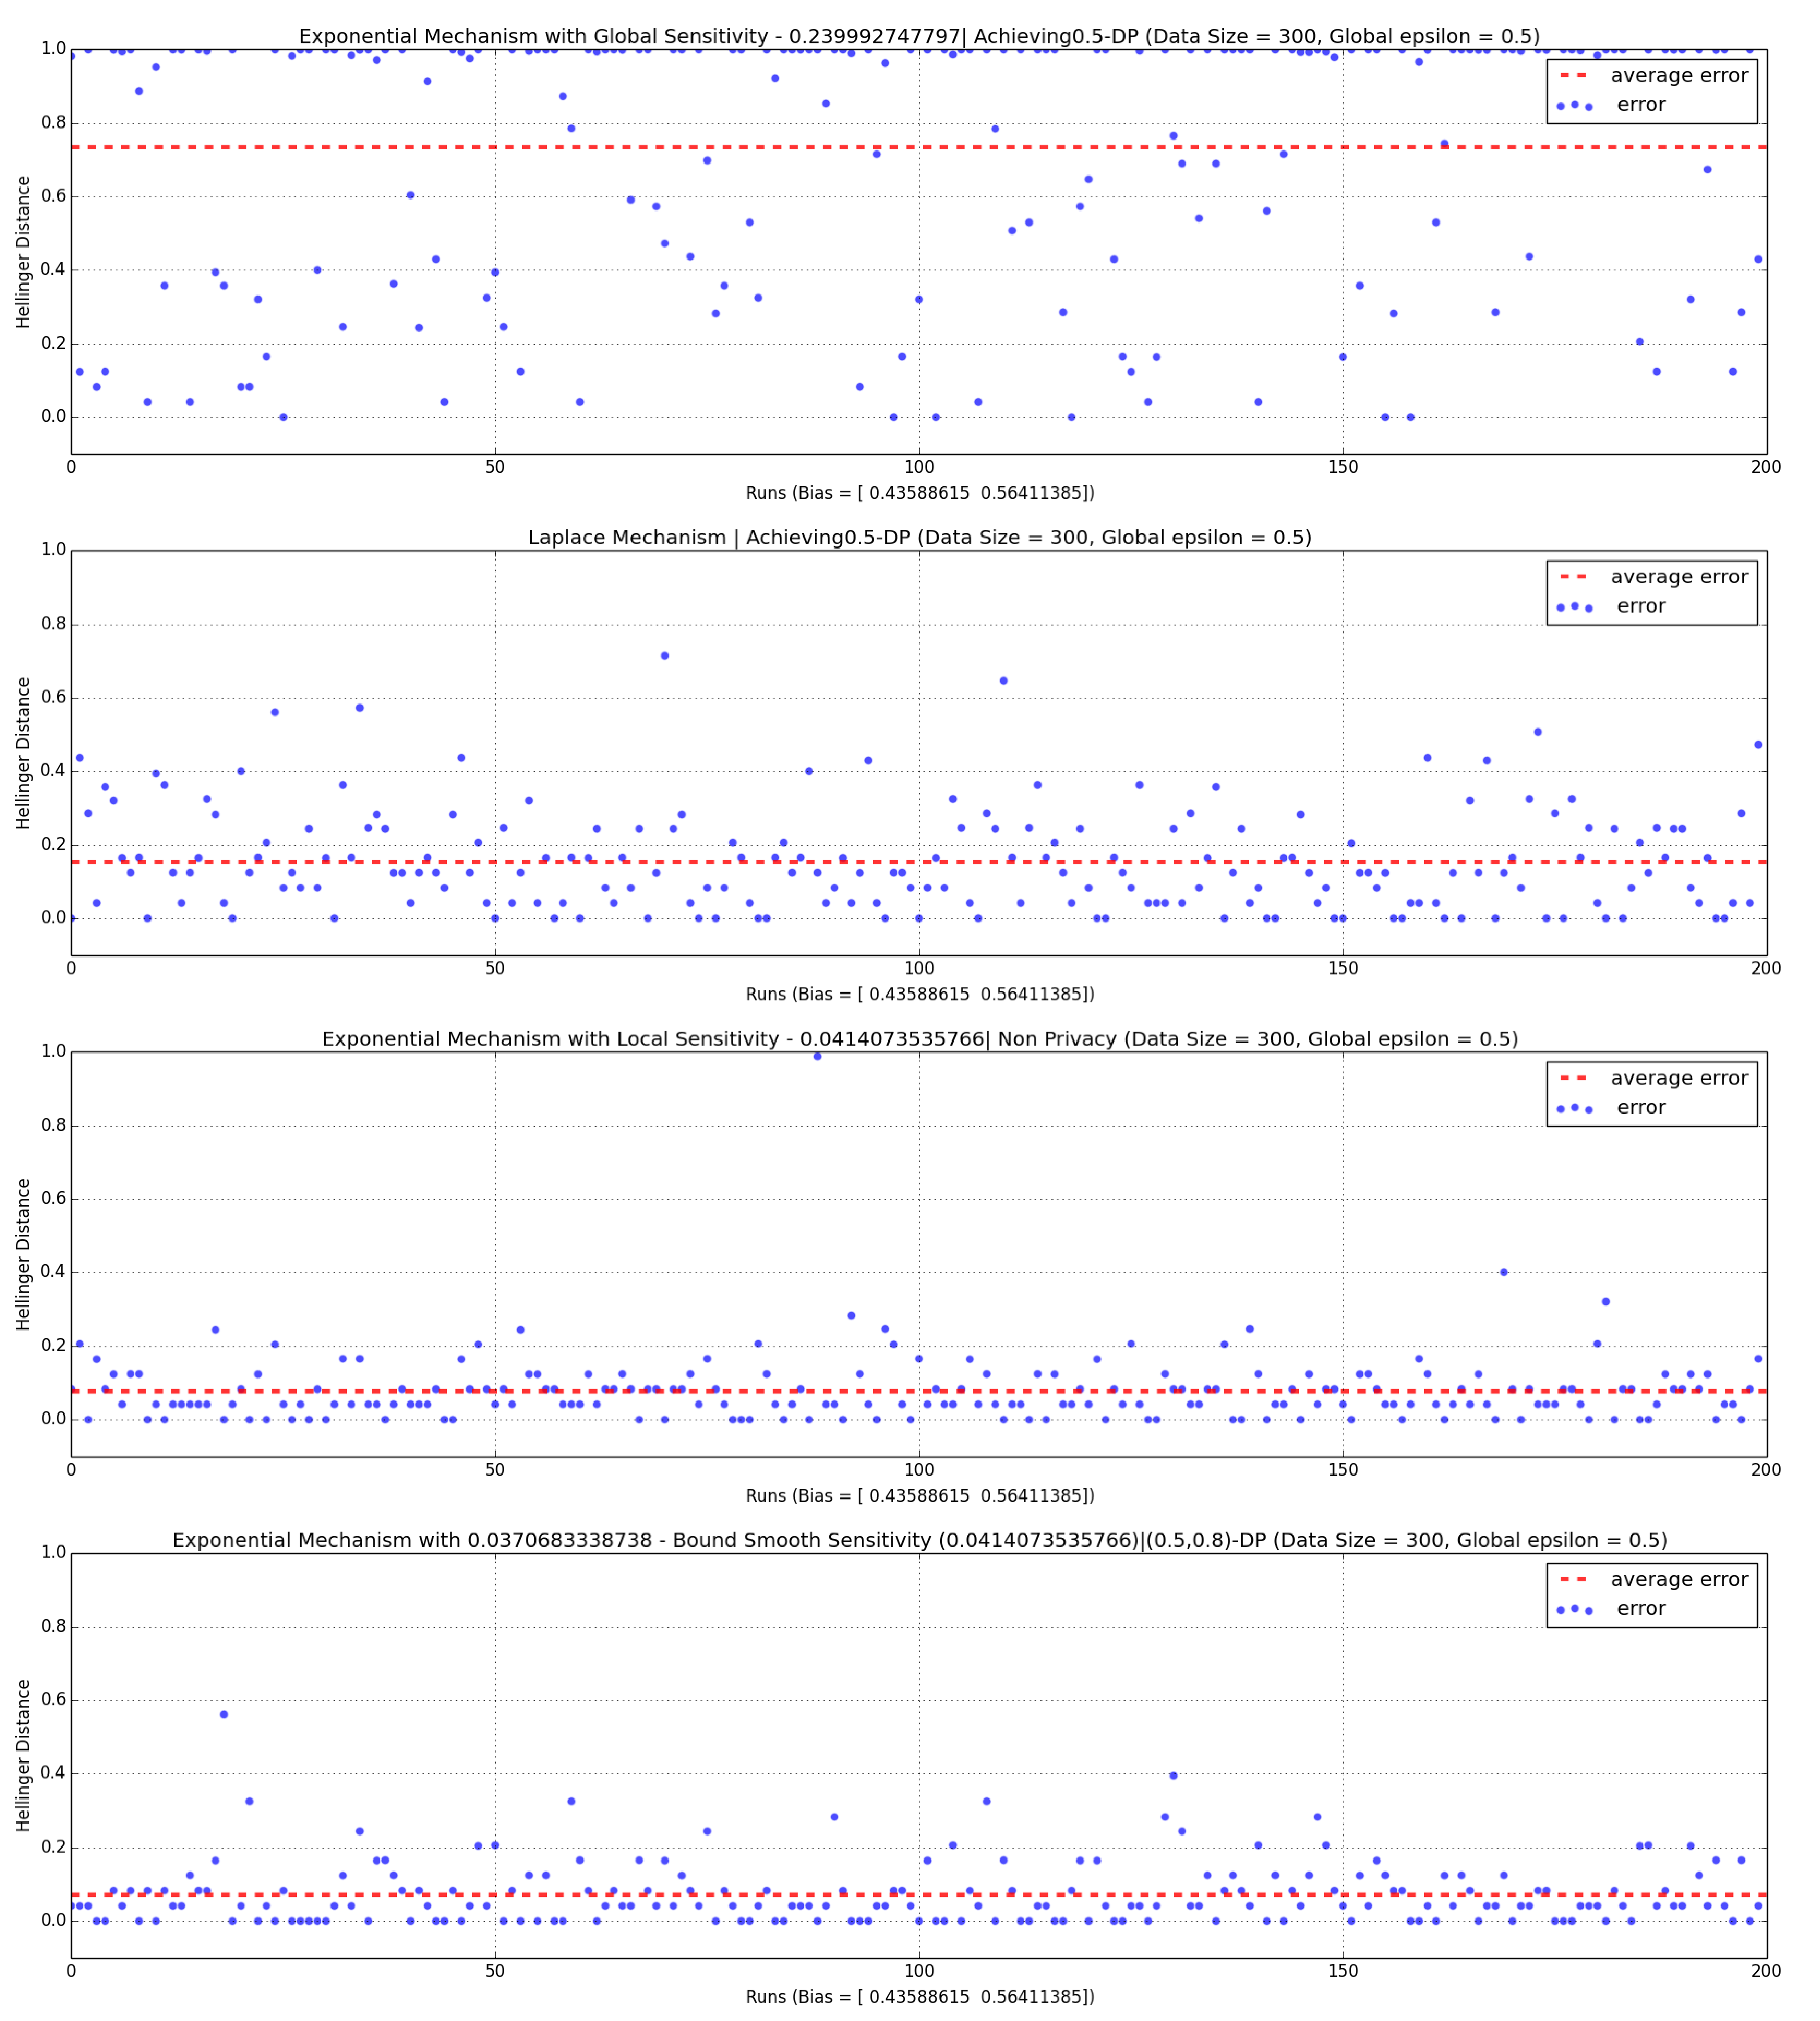
\includegraphics[width=0.48\textwidth]{accuracy_1.eps}}
%   \subfigure[Data size $n = 200$ with global $\epsilon = 0.8$]{
%     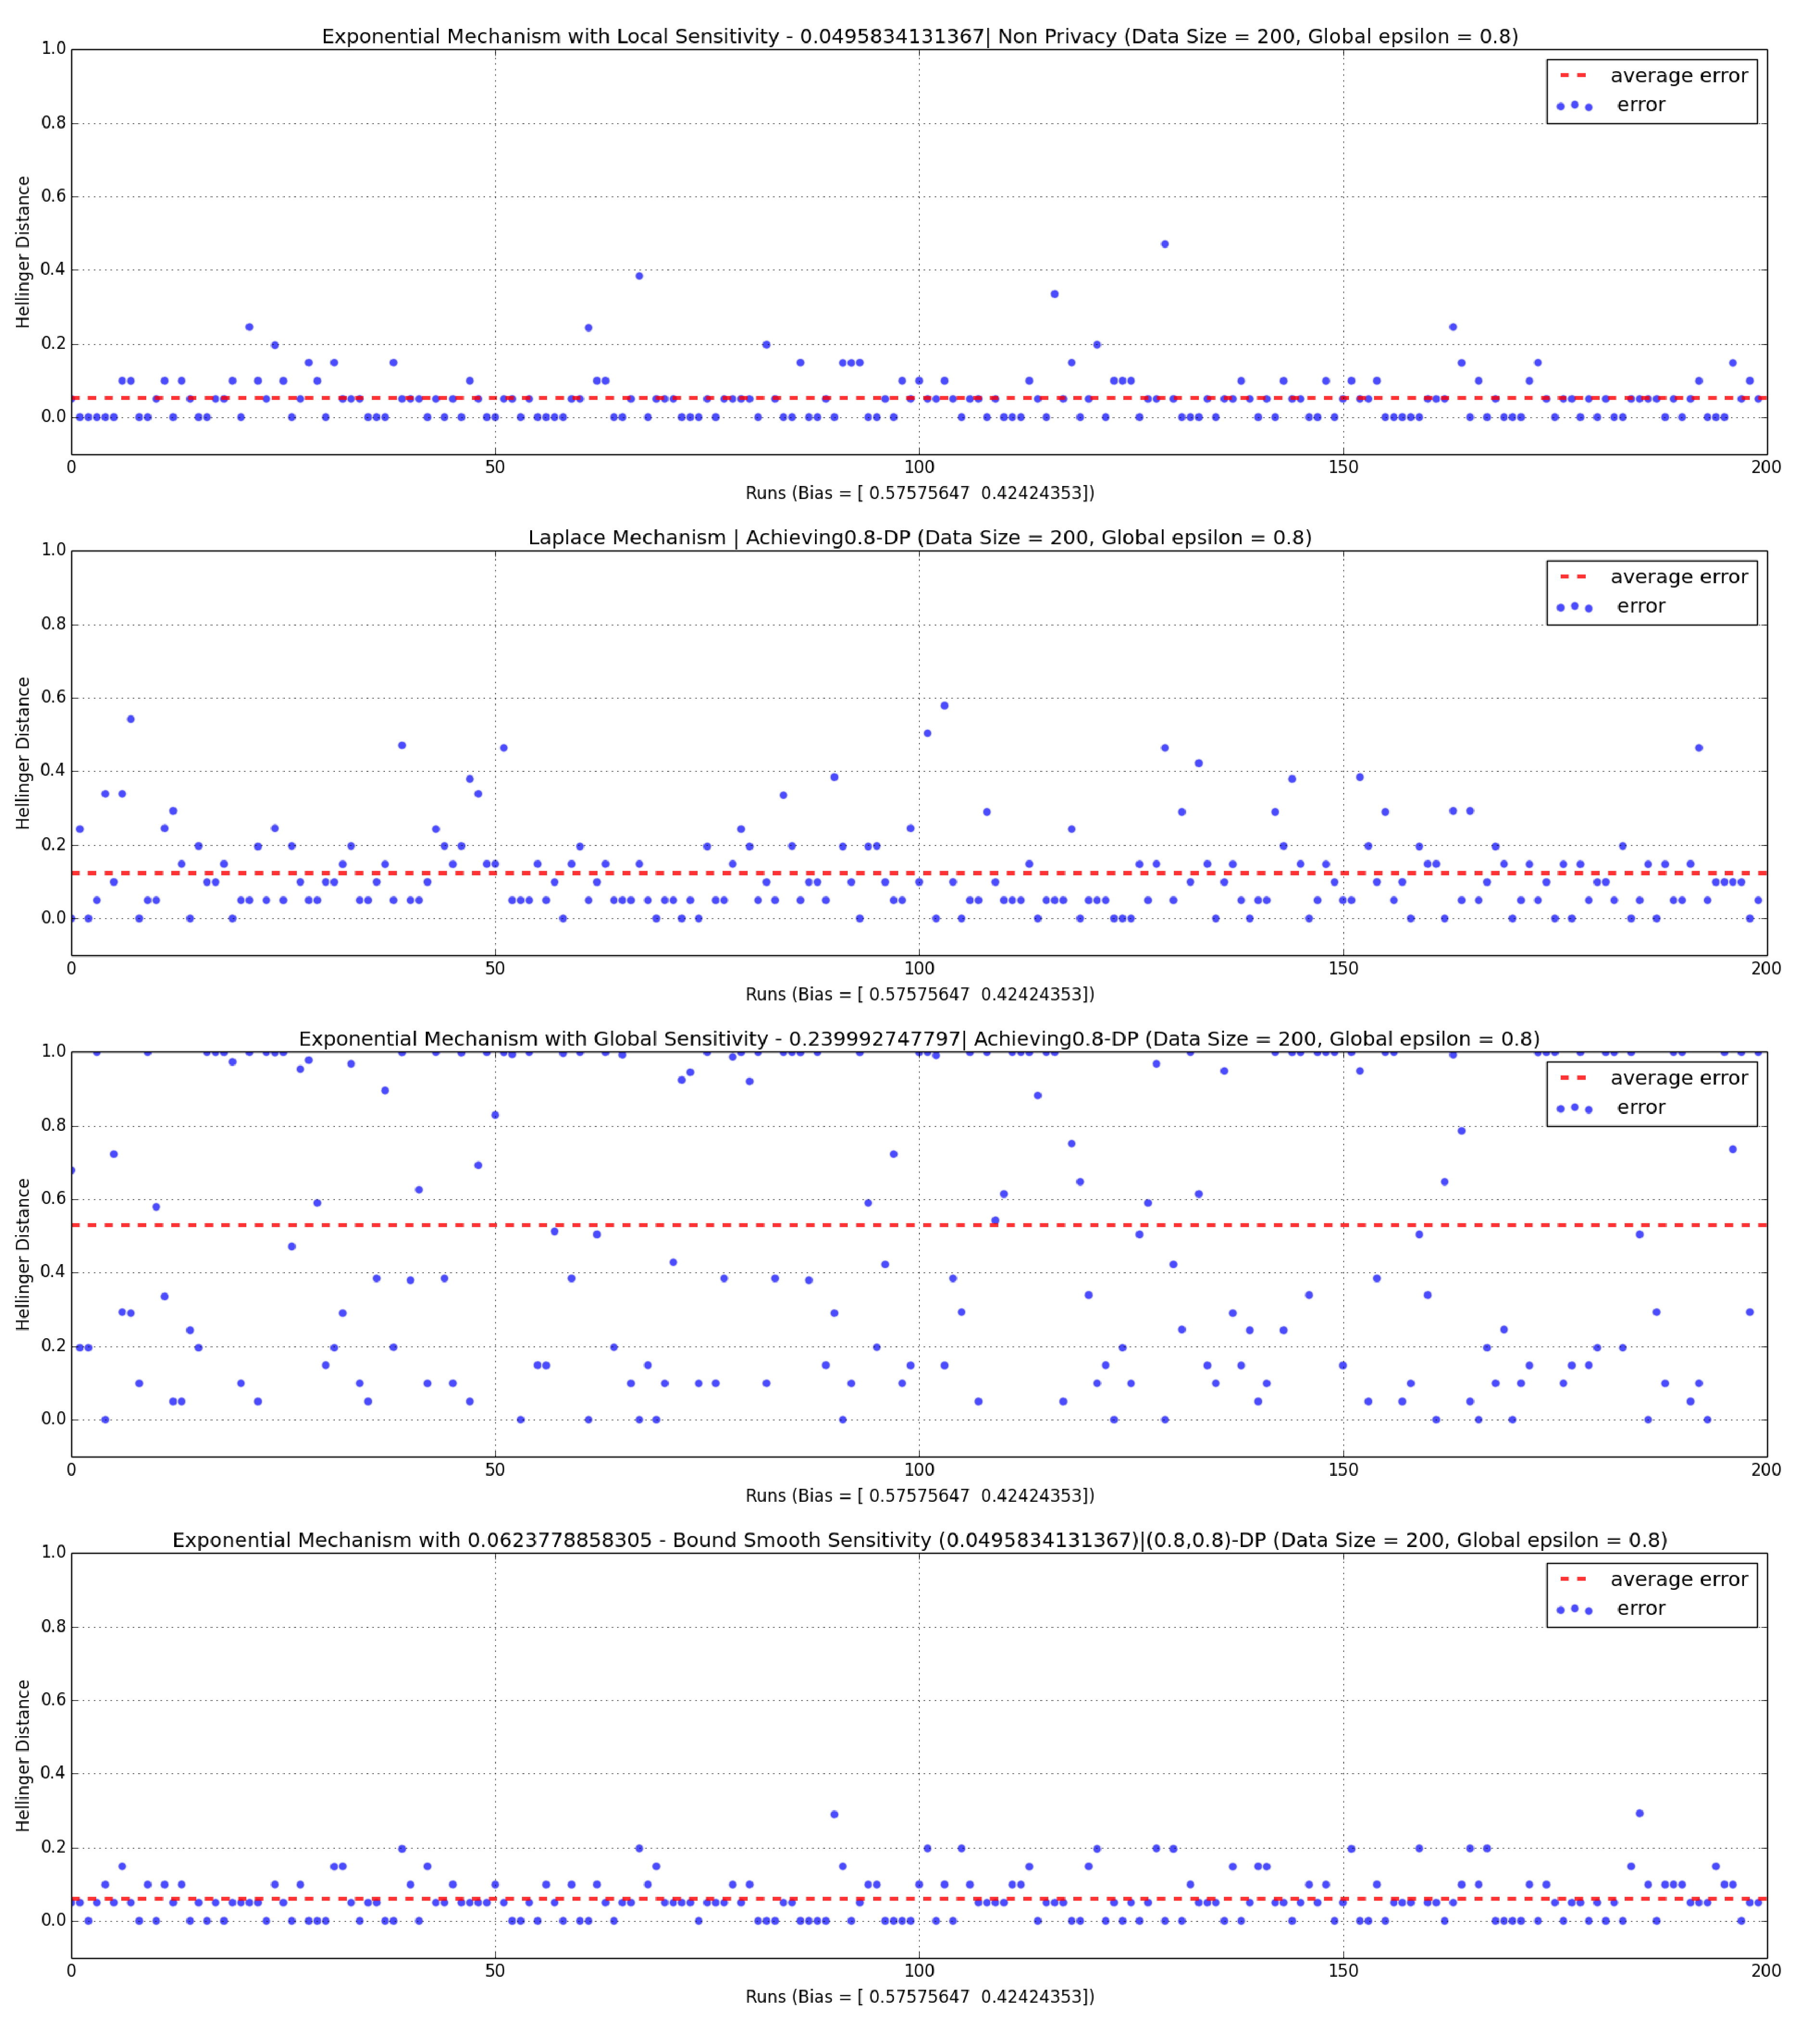
\includegraphics[width=0.48\textwidth]{accuracy_2.eps}} 
% \caption{The experimental results of accuracy of four algorithms}
% \label{fig_data}
% \end{center}
% \end{figure*}

\begin{figure*}
\begin{center}
\centering
  \subfigure[Data size $n = 500$ with global $\epsilon = 0.5$]{
    \includegraphics[width=0.48\textwidth]{accuracy_box_2.eps}}
  \subfigure[Data size $n = 300$ with global $\epsilon = 0.5$]{
    \includegraphics[width=0.48\textwidth]{accuracy_box_1.eps}} 
\caption{The experimental results of accuracy of algorithms with Beta prior distribution $\betad(7,4)$ based on Hellinger distance}
\label{fig_beta_hellinger}
\end{center}
\end{figure*}

We study the accuracy property of the exponential mechanism with three kind of sensitivity, as well as the Laplace mechanism for comparison. As in Fig. \ref{fig_beta_hellinger}, the two figures shown the accuracy of four algorithms under same configuration. The accuracy is measured by Hellinger distance between output $r^*$ and the true inference result $\bysinfer(x)$, $\hlg(r^*, \bysinfer(x))$.

Then, we extended the $\betad$ to the Bernoulli distribution, got the result in Fig. \ref{fig_dirichlet_hellinger}
\begin{figure*}
\begin{center}
\centering
  \subfigure[Data size $n = 100$, the exponential mechanism with global sensitivity 0.239992747797 is 0.8 -DP, with local sensitivity 0.08 is Non-Private and with 0.0699407108115 - bound smooth sensitivity 0.09 is (0.8,0.8)-DP]{
    \includegraphics[width=0.48\textwidth]{accuracy_dirichlet_hellinger_1.eps}}
  \subfigure[Data size $n = 120$, the exponential mechanism with global sensitivity 0.239992747797 is 0.8 -DP, with local sensitivity 0.0945 is Non-Private, with 0.0677791100173 - bound smooth sensitivity 0.096 is (0.8,0.8)-DP]{
    \includegraphics[width=0.48\textwidth]{accuracy_dirichlet_hellinger_2.eps}} 
\caption{The experimental results of accuracy of algorithms with Dirichlet prior distribution $\dirichlet(7, 4, 5)$ based on Hellinger distance}
\label{fig_dirichlet_hellinger}
\end{center}
\end{figure*}


\subsection{Accuracy Study Based on $L_1$ Norm Distance}
For comparison, we study the accuracy of these four mechanisms based on $l_1$ norm, with the Dirichlet distribution $\dirichlet(7,4,5)$ and data size $150$, shown in Fig. \ref{fig_dirichlet_hellinger_l1}.

\begin{figure*}
\begin{center}
\centering
  \subfigure[accuracy measurement based on Hellinger distance]{
    \includegraphics[width=0.48\textwidth]{accuracy_compare_dirichlet_hellinger.eps}}
  \subfigure[accuracy measurement based on $l_1$ norm]{
    \includegraphics[width=0.48\textwidth]{accuracy_compare_dirichlet_l1.eps}} 
\caption{The experimental results of accuracy of algorithms with Dirichlet prior distribution $\dirichlet(7, 4, 5)$ based on Hellinger distance and $l_1$  norm, where data size $n = 150$, the exponential mechanism with global sensitivity 0.239992747797 is 0.8 -DP, with local sensitivity 0.0945 is Non-Private, with 0.0677791100173 - bound smooth sensitivity 0.096 is (0.8,0.8)-DP}
\label{fig_dirichlet_hellinger_l1}
\end{center}
\end{figure*}

\printbibliography

\end{document}

